
\chapter{Algoritmos Evolutivos}

\section{Introducción}

Uno de los puntos importantes del presente trabajo son los algoritmos genéticos por lo que se dedica esta sección para  brindar un repaso por los conceptos y definiciones necesarias para comprender el desarrollo posterior de la solución.

Los algoritmos evolutivos son métodos no determinísticos que se inspiran en la evolución natural de las especies utilizando conceptos como población, cruzamiento, mutación, selección, etc. Estos se utilizan para resolver problemas de optimización y búsqueda, entre otros \citep{Nesmachnow2002}.

Es una técnica iterativa que busca en cada paso mejorar las soluciones por medio de operadores basado en un criterio predefinido para maximizar o minimizar.

Este tipo de solución ha demostrado su utilidad en una amplia variedad de problemas complejos.


\subsection{Algoritmos Genéticos}
El algoritmo genético es uno de los más populares dentro de los algoritmos evolutivos.

La idea base es que partiendo de una población inicial de individuos se seleccionan los mejores en base a su aptitud respecto a solucionar el problema y estos se utilizan para generar nuevos individuos ya sea por combinación o modificación. Por tanto en cada paso obtenemos mejores soluciones hasta detenernos usando un criterio de parada ya sea el número de iteraciones o cuando ya no se puede mejorar más la solución.

Un individuo es una codificación de la solución que resuelve el problema.
La población inicial puede generarse aleatoriamente o basándose en algún conocimiento previo.
La función de evaluación indica que tan buena o apta es una solución en comparación con las demás.
En cada iteración la cual se llama generación se aplican operadores de cruzamiento estos son formas de combinar a los individuos para obtener otros que potencialmente sean una mejor solución y también cambios aleatorios sobre los individuos llamado mutación.

Por tanto se van seleccionando, combinando y cambiando las mejores soluciones en un proceso que va obteniendo mejores soluciones.
El criterio de parada nos indica cuando termina este proceso, ya sea por que se alcanzó un número de generaciones predefinidos o por que la mejora no es evidente. Al final se devuelve la mejor solución encontrada en todo el proceso.

Hay que indicar que no es una técnica exacta pero si logra muy buenas aproximaciones y es muy buena en problemas complejos por su flexibilidad y robustez. 


\subsubsection{Representación de soluciones}
No podemos trabajar directamente sobre las soluciones, por lo que tenemos que codificarlas en un modelo que nos sirva para poder aplicar el algoritmo.
La inspiración biológica se ve en los nombres que adopta esta representación, llamada Cromosoma que es un vector de genes y cada valor de un gen se llama alelo.
En general se codifica un vector de números binarios o reales de largo fijo, lo que facilita la aplicación de los operadores.

\subsubsection{Función de Evaluación} 
Indica que tan bueno es un individuo para resolver el problema en cuestión con un valor conocido como Fitness. Este se utiliza para seleccionar a los mejores y de esta forma guiar la exploración hacia la mejor solución.
Se deben tener en cuenta las restricciones del problema para que las soluciones no factibles no sobrevivan.
En general es donde se consume el mayor tiempo del algoritmo en comparación con los demás operadores.

\subsubsection{Operador de Selección}
Existen diversos operadores de selección , su función es que las mejores características de los individuos se mantengan en las siguientes generaciones.
Los tipos más populares son:

\begin{itemize}
	\item Ruleta: También conocida como selección proporcional elige aleatoriamente individuos en la cual la probabilidad de selección es proporcional al valor de fitness.
	\item Torneo: Se elige aleatoriamente un determinado número de individuos los cuales compiten entre si.
	\item Elitismo: Los mejores individuos son mantenidos entre las generaciones.
\end{itemize}

\subsubsection{Cruzamiento}
Su función es combinar individuos para lograr mejores soluciones. 
Existe una tasa que se puede modificar para indicar la probabilidad de que se realice el cruzamiento.

\begin{itemize}
	\item Cruzamiento de un punto: A partir de dos padres se selecciona un punto al azar de los cromosomas obteniendo dos trozos que se combinan para obtener dos hijos. Se explica en la figura ~\ref{fig:cruzamiento1}
	\item Cruzamiento multipunto: El método anterior se puede generalizar para obtener más puntos de corte y más recombinaciones.
\end{itemize}

\begin{figure}[h]
\centering
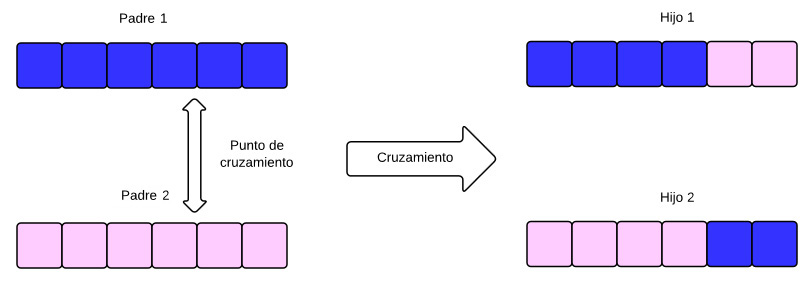
\includegraphics[width=\textwidth]{Figures/cruzamiento1}
\caption{Cruzamiento de un punto}
\label{fig:cruzamiento1}
\end{figure}

\subsubsection{Mutación} 
Indica el método utilizado para modificar un individuo, esto se realiza para lograr más diversidad y no caer en máximos locales. En general aplica una modificación aleatoria en el cromosoma.También hay una tasa de probabilidad, en general es baja. En el caso de un cromosoma binario se aplica la inversión sobre un alelo.

\begin{figure}[h]
\centering
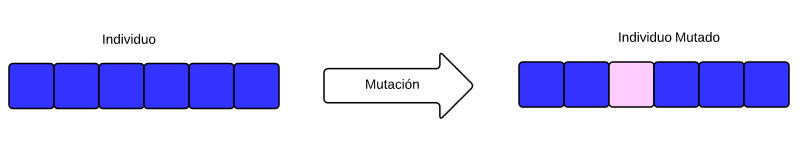
\includegraphics[width=1\linewidth]{Figures/mutacion1}
\caption{Mutacion por inversión binaria}
\label{fig:mutacion1}
\end{figure}


\subsubsection{Reemplazo} 
Se indica cual es el criterio que debemos tomar para generar una nueva población, ya sea tomando solo los hijos creados o comparando también con los padres o aplicando algún otro criterio.

\subsubsection{Criterio de parada} 
Indica cuando debe terminar el algoritmo, puede ser definiendo un número fijo de generaciones o analizando si el mejor valor de fitness se mantiene relativamente constante durante un número determinado de generaciones.

\subsection{Funcionamiento}

El esquema básico de funcionamiento es el siguiente:


\begin{algorithm}%[!ht]
	\caption{Algoritmo Genético}
	\label{alg:algoritmo_genetico_simple}
	\begin{algorithmic} [1] 
		{
			%\small
			\STATE {Inicializo( Pob(0))}
			\STATE \texttt{generacion} = 0
			\WHILE {\text{No llegue al criterio de parada}}
			\STATE {Evaluar Pob(generacion)}
			\STATE {Padres = Seleccionar(Pob(generacion))}
			\STATE {Hijos = Cruzamiento(Padres) y Mutacion(Padres)}
			\STATE {NuevaPob = Reemplazar Pob(generacion) con Hijos}
			\STATE \texttt{generacion}++
			\ENDWHILE
			\RETURN Mejor solución
		}
	\end{algorithmic}
\end{algorithm}




\subsection{Algoritmos genético multiobjetivo}

En este caso se busca una solución que satisfaga de forma simultánea tanto las restricciones del problema como varios objetivos distintos.



\subsection{Algoritmo Genético Paralelo}
Los problemas complejos suelen requerir una alta demanda computacional por lo que aplicar técnicas de paralelización es útil para lograr tiempos de ejecución menores.

Existen varios niveles de paralelización ya sea a nivel global enfocándonos en paralizar la función fitness, a nivel de la población, o a nivel del individuo. \citep{Nesmachnow2002}

En el caso de los algoritmos genéticos gran parte del tiempo se ocupa en la etapa de evaluación, por esta razón es un buen método para distribuir la carga en varios procesadores para que las evaluaciones se realicen en paralelo.


\subsection{Maestro-Esclavo}

En este modelo un proceso maestro es el encargado de realizar los operadores básicos del algoritmo y distribuir a procesos esclavos la evaluación de la función fitness para un conjunto de individuos, el esclavo devuelven el resultado y luego el maestro es el encargado de continuar ejecutando los operadores.

De este modo aumenta la eficiencia computacional del algoritmo ya que una de las funciones más costosas es distribuida entre varios nodos.

\begin{figure}[H]
\centering
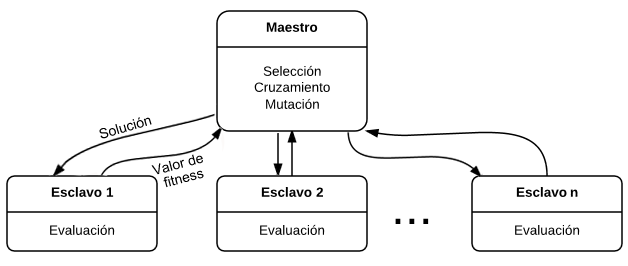
\includegraphics[width=0.7\linewidth]{Figures/diagrama-master-slave}
\caption[Modelo Maestro-Esclavo]{Modelo Maestro-Esclavo}
\label{fig:diagrama-master-slave}
\end{figure}

